\section{Aproximando funciones con neuronas}

\noindent
En computación, la palabra \emph{aprendizaje} es sinónimo de ``minimización de\
errores'', lo que lleva a cuestionarnos la existencia de una conexión entre\
este fenómeno estadístico con las maneras que, naturalmente, posee el cuerpo humano\
para comprender de su medio ambiente. Concretamente, la tarea que tiene el computólogo\
ante sí consiste en transformar los problemas de aprendizaje automático en\
equivalentes compatibles con el funcionamiento del sistema nervioso humano. Dadas,\
las evidencias empíricas sobre el buen desempeño del cerebro humano en su cotidianidad,\
nos inspiramos en el comportamiento biológico del mismo para construir arquitecturas\
cuyo objetivo será el de aproximar funciones complejas, creando un novedoso paradigma de cómputo.\par
Con el fin de ilustrar al buen \emph{performance} del cerebro humano, consideremos a las\
habilidades de reconocimiento perceptivo. Mientras una persona tarda de $100$ a $200$ $ms$\
en detectar un rostro familiar, una computadora con suficiente poder dura mucho más.\cite{haykin2009}\
En contraste, se sabe que individualmente, una neurona es mucho más lenta que una\
compuerta lógica: mientras que ésta últimas tardan pocos nanosegundos en \emph{conmutar},\
a la primera mencionada le puede tomar varios milisegundos en reaccionar a un estímulo.

\subsection{Inspiración a partir de la biología}

\noindent
El sistema nervioso es una red \emph{paralela} y \emph{auto-organizada}. $86$ mil\
millones de neuronas (aproximadamente) \cite{website:nature:scitable} conforman una arquitectura que\
funciona a través de la emisión de pulsos eléctricos y la reacción ante ellos. Dos neuronas\
están conectadas entre sí por medio de estructuras conocidas como \emph{sinapsis},\
a través de las cuales se transmiten señales eléctricas y químicas.\par
El cerebro es, además, un órgano que se adapta a las condiciones de su ambiente.\
Evidencia de ello es la creación de conexiones sinápticas entre neuronas (previamente\
desconectadas) y la modificación del mecanismo de las sinapsis existentes. Una vez que una\
neurona haya emitido una señal eléctrica, las adyacentes reciben la \emph{``información''}\
por medio de canales de transimisión llamados \emph{dendritas}. Estos impulsos son llevados\
hasta el \emph{cuerpo} de la neurona para su procesamiento y, posteriormente, una reacción\
es transmitida a través del \emph{axón} de la célula. Los organelos mencionados anteriormente\
constituyen las principales partes de la neurona que habrán de servir como estructuras\
fundamentales de las arquitecturas de aprendizaje a presentar en las siguientes secciones.\cite{rojas1996}

\begin{figure}[H]
  \centering
  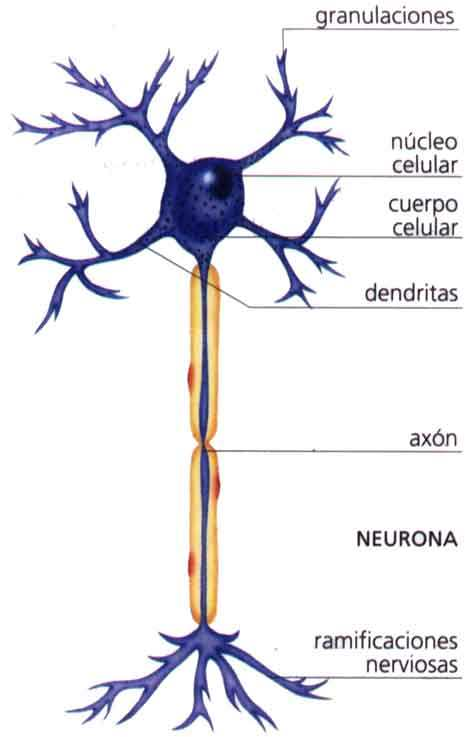
\includegraphics[width=\textwidth, height=0.6\textheight]{neurona}
  \caption{Ilustración de las partes más importantes de una neurona humana.
    (Tomado de (\url{https://psi121f.wordpress.com/2016/07/03/la-estructura-de-la-neurona-2/}))}
\end{figure}


\subsection{El modelo de cómputo neuronal}

Dadas varias entradas eléctricas, una neurona deberá de ajustar su reaccion de manera proporcional\
a la intensidad de las dichas señales. Para formalizar el comportamiento de una neurona en términos\
matemáticos (y, por ende, computacionales), es imprescindible caracterizar las reglas que sigue una neurona\
para componer sus señales de entrada y manejarlas ``globalmente'' mediante una función. Cabe destacar\
que, por simplicidad y elegancia de los modelos a estudiar, resulta importante conocer la \emph{sincronía}\
de la transmisión de información así como la presencia o ausencia de ciclos o bucles. Todo esto se puede\
englobar en un conjunto de características topológicas y algorítmicas que constituyen a una \emph{red neuronal artificial}\
(ANN, por sus siglas en inglés; en adelante, abreviaremos ANN con NN).\par
Con respecto a la representación interna del conocimiento de una NN, estamos ante un conjunto de modelos\
que buscarán modelar la información de manera \emph{asociativa}; análogamente al cerebro humano. Por ende,\
se requieren modelos que \emph{relacionen} clasificaciones de objetos similares con representaciones internas\
similares. Con el fin de asegurarnos de ello, presentaremos más adelante una completa sección\
acerca de métodos de mediciones de similitud. Una consecuencia importante de esto es que,\
de manera contraria, si se desea que dos objetos sean distintamente clasificados,\
entonces se les deben de dar dos representaciones totalmente diferentes.\par
Independientemente de la tarea que se desea aprender, siempre existirá alguna característica cuya importancia\
define el veredicto de la NN. Una forma de respaldar este hecho consiste en dedicar un gran\
número de neuronas a la identificación de dicha característica. Con ello, se aumenta la\
precisión de la NN en su toma de decisiones, contrastando con la existencia de neuronas defectuosas.\par
Finalmente, la existencia de un \emph{zoológico de redes neuronales} se justifica con la tendencia\
que se sigue a diseñar modelos específicos para ciertas tareas. Si se sabe información \textit{a priori}\
sobre los datos a procesar, es mejor integrarlas en el diseño de la arquitectura a dejar que ésta\
los aprenda durante el entrenamiento. Después de todo, en el cuerpo humano existen una gran cantidad\
de estructuras neuronales especializadas para funciones como visión y audición, muy distintas a otras\
presentes en el cerebro.

\subsection{El perceptrón de Rosenblatt}

\noindent
La idea de cómputo a través de redes neuronales fue tan trascendente desde su concepción, que, en 1943,\
McCulloch y Pitts la incluyeron en el mismo artículo que introdujo a los sistemas de transición con un número\
finito de estados \cite{mcculloch:pitts}. Sin embargo, fue Rosenblatt, en 1958, quien propuso el primer modelo de aprendizaje supervisado para una NN.\
El perceptrón es la red neuronal más simple y, muchas veces, será uno de los bloques básicos de arquitecturas\
más complejas. La intuición matemática detrás de su estructura consiste en \emph{separar linealmente} las entradas dadas en\
dos clases, lo cual se logra mediante un aprendizaje que va ajustando pesos de acuerdo a las salidas esperadas.\par

\begin{figure}[H]
  \centering
  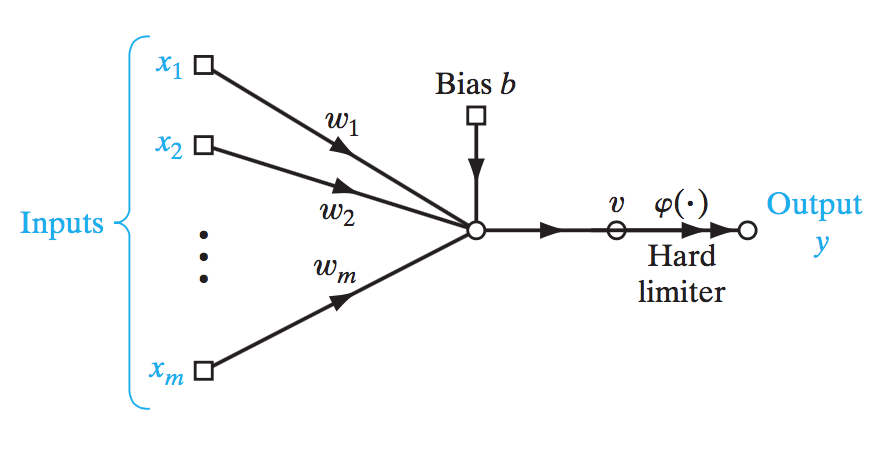
\includegraphics[width=\textwidth]{perceptron}
  \caption{El perceptrón de Rosenblatt es un modelo gráfico cuya salida depende de las contribuciones
    lineales de cada una de las entradas, de un sesgo y de una función no lineal de activación.
    (Tomado de \cite{haykin2009})}
  \label{perceptron-fig}
\end{figure}


De acuerdo a la Figura \ref{perceptron-fig}, el perceptrón opera de la siguiente manera: dados los valores\
de entrada $x_1, x_2,\ldots, x_m$ y los pesos $w_1, w_2,\ldots, w_m$,
\begin{itemize}
\item se calcula una suma ponderada con los $m$ pesos (\emph{sinápticos}) del modelo,
\item a la suma anterior, se le añade un valor de \emph{``tendencia''} conocido como \emph{sesgo}\
  (\emph{bias} en inglés); formalmente:
  \begin{equation}
    v = b + \sum_{i=1}^{m} w_ix_i
  \end{equation}
\item finalmente, la salida del perceptrón se calcula aplicando una función \emph{de activación} a $v$:
    \begin{equation}
      y = \Phi(v).
    \end{equation}
\end{itemize}

La función de activación juega el papel directo de clasificador: su salida debe de decidir si la entrada\
pertenece, o no, a cierta clase. De ahí que en la mayoría de los casos, se trata de una función cuya imagen\
es $\{0,1\}$ o $\{-1,1\}$. Por otra parte, dado que estamos definiendo al perceptrón con operaciones\
aritméticas como sumas y productos, cabe recalcar que las entradas deben ser una \emph{abstracción numérica}\
del elemento del entorno a clasificar; muchas veces ésta se compone de un vector de valores reales. Ello implica\
la existencia de un \emph{umbral} $U$ (\emph{threshold} en inglés) que divida los posibles valores de $v$\
en dos, permitiendo su clasificación binaria. A continuación, se define la \emph{función escalón}, valuada\
en $\{-1,1\}$ (una posible función de activación):
\begin{equation}
  \Phi(v) =
  \begin{cases}
    1 & \text{si } v > U\\
    -1 & \text{en otro caso}
  \end{cases}
\end{equation}
Geométricamente, el perceptrón genera un \emph{hiperplano} que, con los pesos adecuados logrará dividir\
las entradas de manera que cada entrada correspondiente a una cierta clase quede dentro de \emph{una y sólo una}\
partición del espacio multidimiensional en cuestión.\par
El hecho de que estamos usando funciones de activación valuadas de manera binaria nos invita a explorar el\
cómputo \emph{neuronal} de las diversas funciones lógicas. Como ejemplo, está la clasificación de\
la función \verb+OR+ en la Figura \ref{or-fig}. En este caso, se tienen entradas de dos dimensiones, por lo que es\
posible visualizarlas gráficamente; en la práctica, se trabaja con un gran número de dimensiones, de lo cual\
se deduce la importancia de tomarán algunos métodos de reducción dimensional para el éxito de los algoritmos\
de entrenamiento de modelos más complejos.\par

\begin{figure}[H]
  \centering
  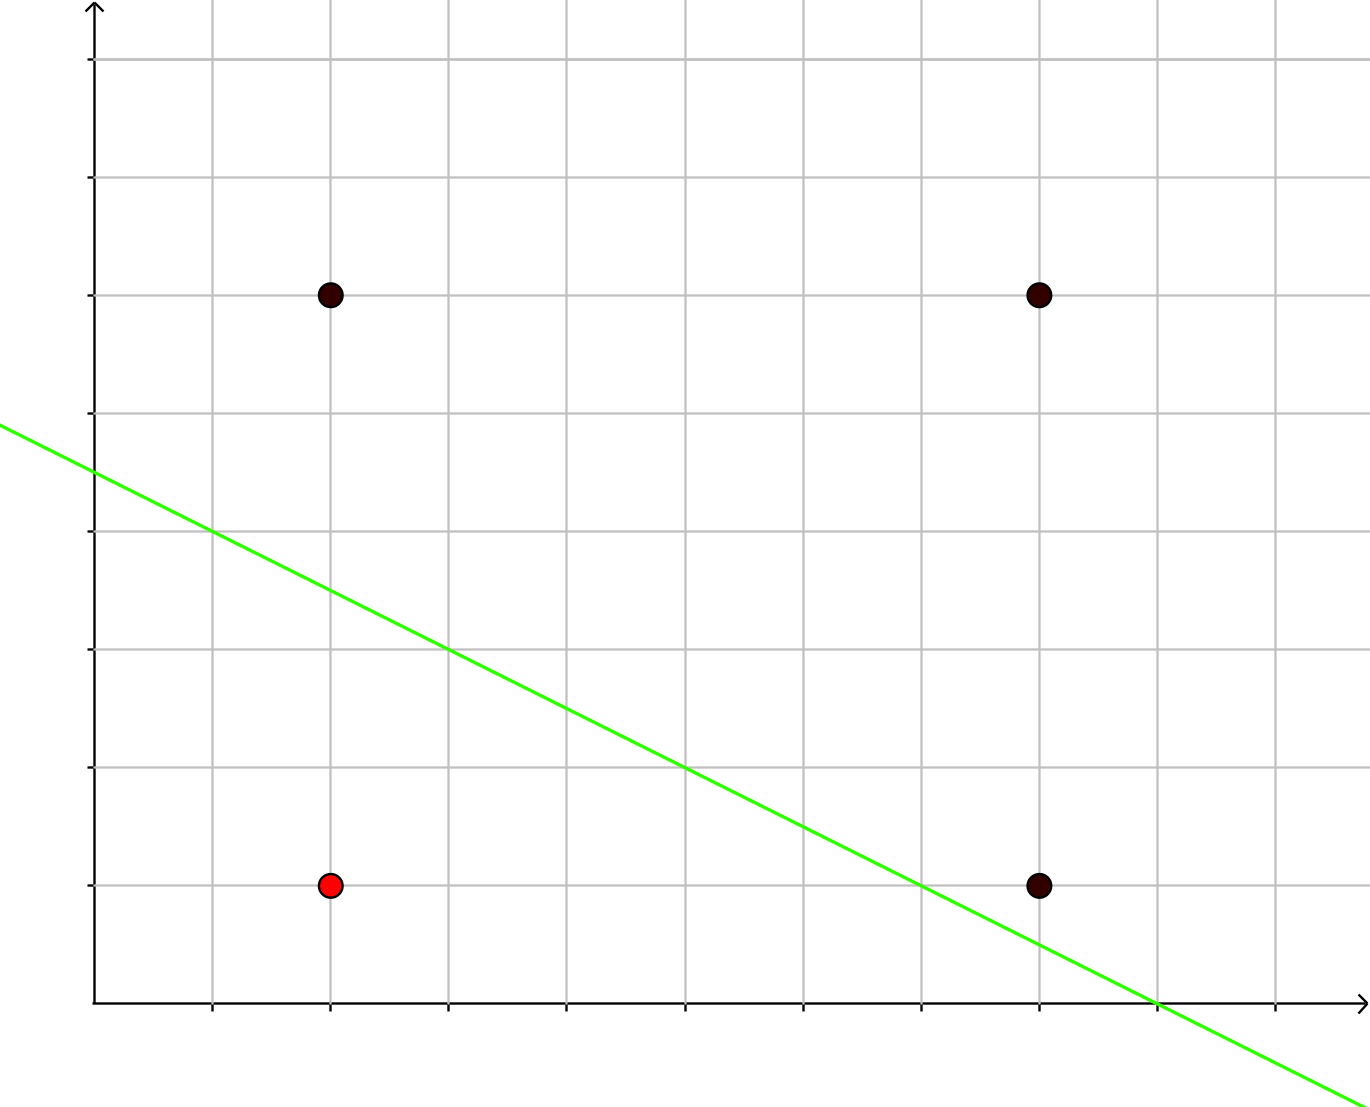
\includegraphics[width=\textwidth]{or}
  \caption{La función lógica \texttt{OR}, en su versión bidimensional, tiene cuatro posibles salidas:
    tres de ellas arrojan un valor positivo, mientras que la otra es negativa. Claramente, se trata de una función
    separable mediante una recta.
    (Elaboración propia.)}
  \label{or-fig}
\end{figure}

Para finalizar esta sección, cabe destacar que la función de activación ($signo$) que acaba de ser presentada\
no es la única. En realidad, se buscan opciones más suavizadas y, sobre todo, diferenciables con el fin de\
optimizar los parámetros de modelos más complejos.

\begin{figure}[H]
  \centering
  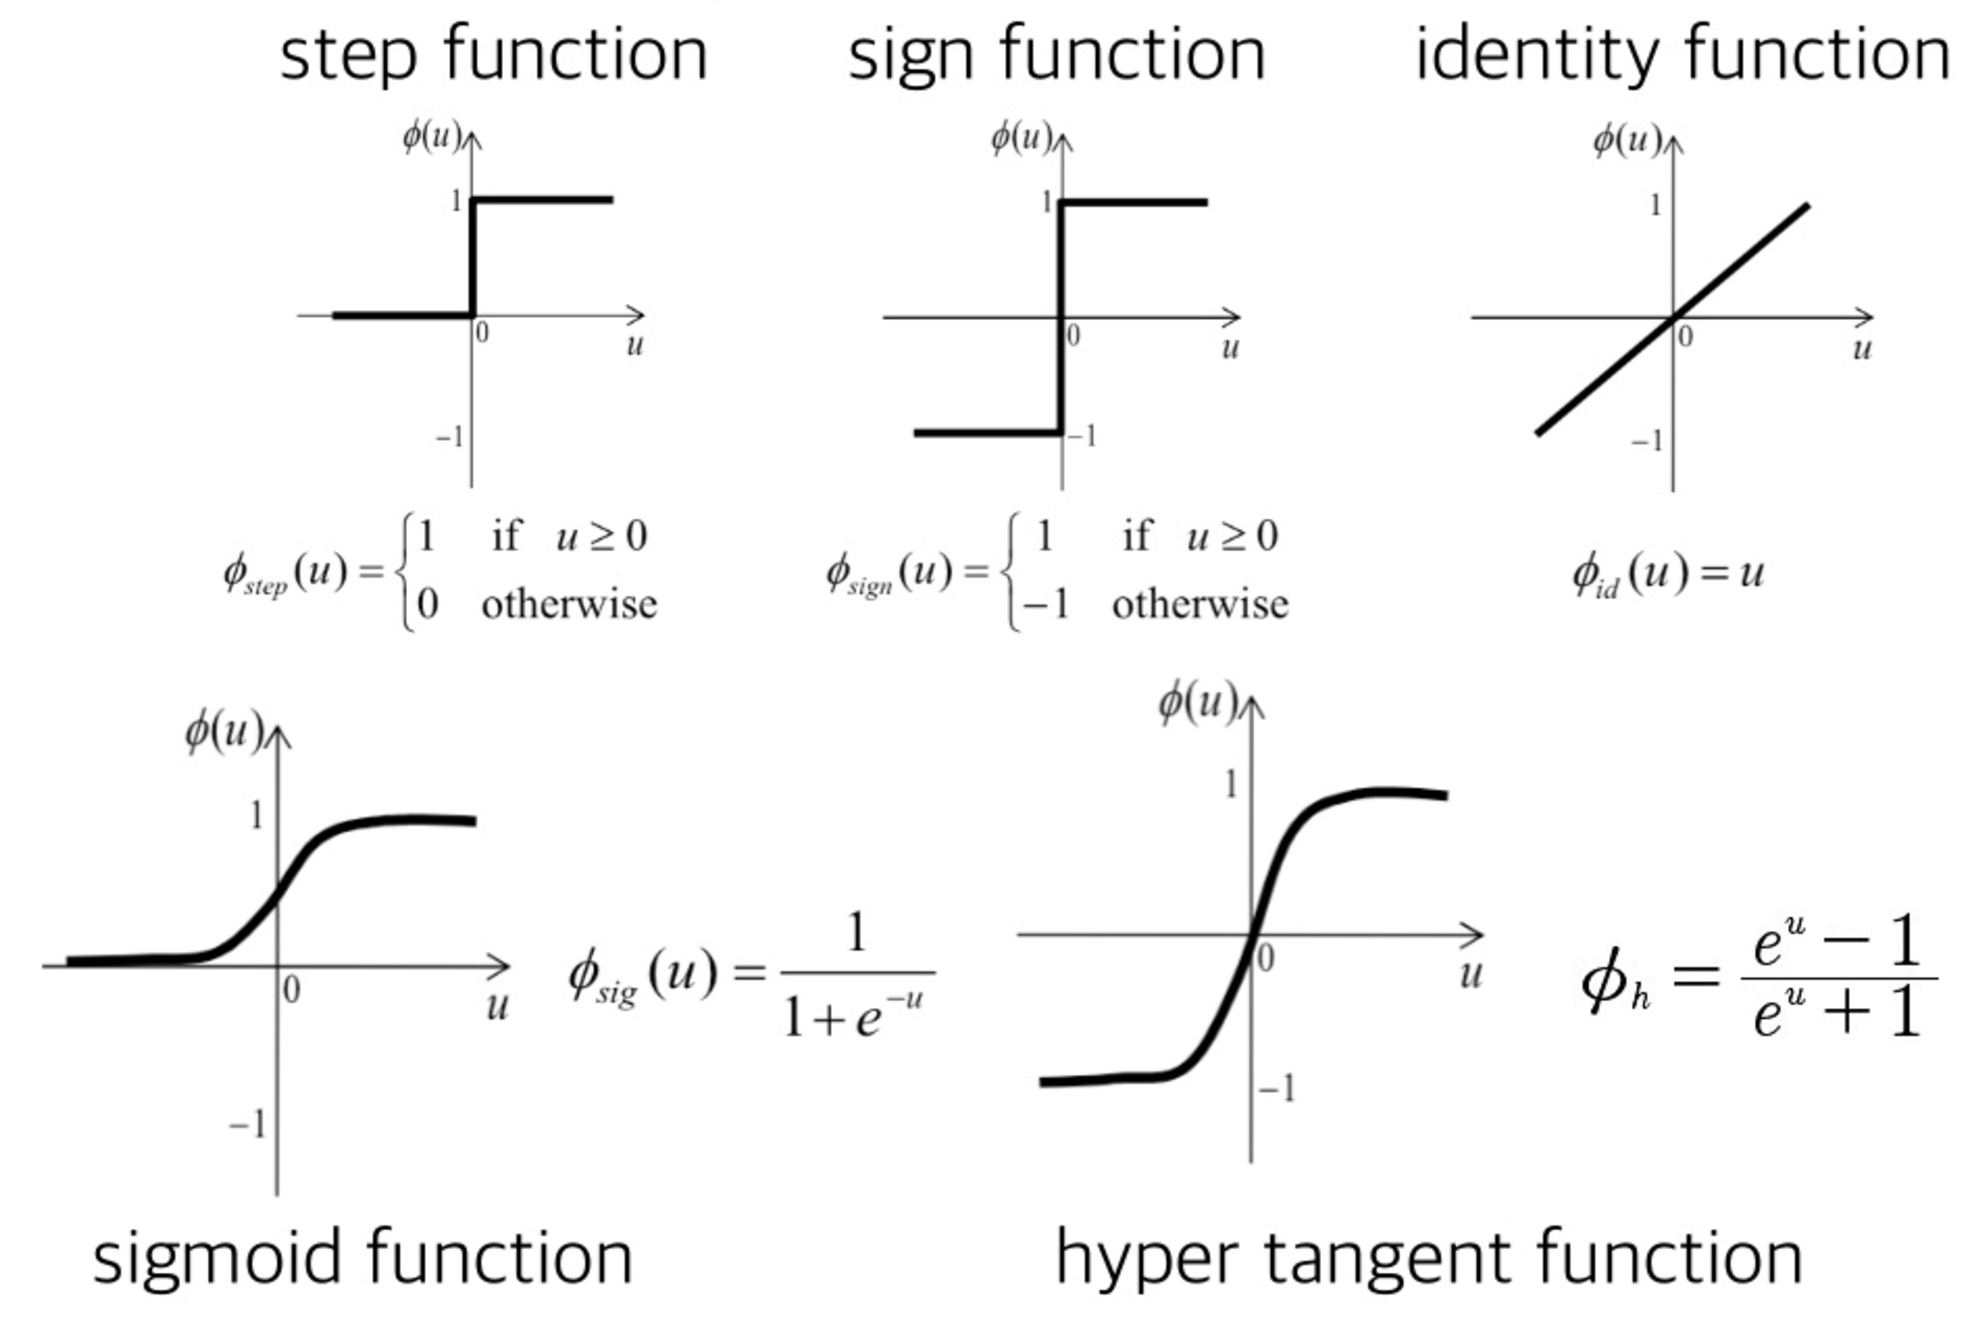
\includegraphics[width=\textwidth]{activations}
  \caption{Las funciones de activación más comunes.
    (Tomado de (\url{https://www.slideshare.net/SungJuKim2/multi-layer-perceptron-back-propagation}))}
\end{figure}

\subsection{El perceptrón multicapa}

\noindent
No todos los patrones de datos son linealmente separables. Por ejemplo, la función lógica \verb+XOR+, contiene\
salidas cuyos valores no pueden ser divididos en dos partes del plano sin ser mezclados. Por consiguiente,\
es necesario aumentar la capacidad de cómputo del perceptrón. Combinaremos, ahora, varios perceptrones\
en una \emph{red neuronal de propagación hacia adelante}, estructurando el cómputo en distintas\
\emph{capas ocultas}.\par
El flujo de la información irá de capa en capa, en una sola dirección hasta llegar a una \emph{capa de salida}.
Cada capa oculta consta de un conjunto de neuronas, sin conexiones entre ellas, pero totalmente conectadas a la\
capa inmendiatamente anterior y posterior. A este modelo se le conoce comúnmente como\
\textbf{perceptrón multicapa} (\emph{MLP} por sus siglas en inglés) y es el punto de partida de la rama\
del aprendizaje automático conocida como \textbf{aprendizaje profundo} (\emph{deep learning} por sus siglas en inglés).

\begin{figure}[H]
  \centering
  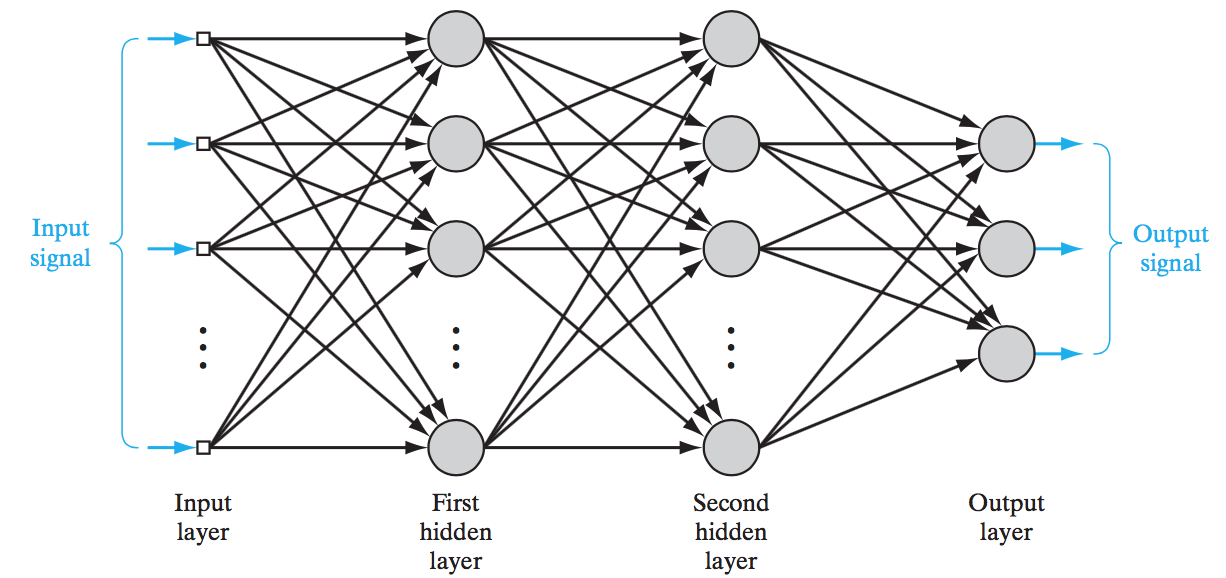
\includegraphics[width=\textwidth]{mlp}
  \caption{Arquitectura de un MLP con dos capas ocultas.
    (Tomado de \cite{haykin2009}.)}
\end{figure}

El flujo del cómputo en un MLP puede ser pensado como la composición de las capas ocultas, vistas como funciones que\
procesan los datos de entrada. Formalmente, dado un vector de entrada $\mathbf{x}$, la primera capa oculta $h_1$\
calcula su valor utilizando una matriz de pesos $\mathbf{W_1}$, un sesgo $\mathbf{b_1}$ de la siguiente manera:
\begin{equation}
  h_1 = \sigma\left(\mathbf{W_1}^\top \mathbf{x} + \mathbf{b}_1\right),
\end{equation}
donde $\sigma$ es una función de activación no lineal y \emph{diferenciable}.\
Las dimensiones de $\mathbf{W}$ corresponden a la entrada y al número de neuronas en la capa $h_1$.\
La $i+1$-ésima capa oculta de un MLP actualiza su valor a partir de la $i$-ésima mediante
\begin{equation}
  h_{i+1} = \sigma\left(\mathbf{W_{i+1}}^\top h_i + \mathbf{b}_{i+1}\right),
\end{equation}
es decir, cada capa tendrá una matriz de pesos y un vector de sesgos propio. La salida, suponiendo que\
hay $m$ capas ocultas, obtiene su valor con la equación
\begin{equation}
  \hat{y} = \sigma\left(\mathbf{W_{m+1}}^\top h_m + \mathbf{b}_{m+1}\right).
\end{equation}
Obsérvese que es posible que $\hat{y}$ tenga más de una dimensión, entonces, cada uno de los valores de dicho\
vector codificará ``la existencia'' de alguna característica en particular. Esto es muy útil para aprender\
clasificadores cuyo contra-dominio es mayor al conjunto binario.\par
En ocasiones, al subrafo dirigido formado por las capas ocultas $h_i$ y $h_{i+1}$ se le conoce como\
\emph{capa densa} o \emph{totalmente conectada} y es común encontrarla en arquitecturas de mayor complejidad\
y especialización. El MLP está dentro del ``estado del arte'' de los algoritmos de clasificación automática y\
será parte fundamental de los dos modelos neuronales que compone a la arquitectura de procesamiento de imágenes\
y generación de lenguaje de la presente tesis. La parte más importante de ello recae en su algoritmo de\
aprendizaje que a continuación se describe.

\subsection{Retroalimentación para aprender}
